\documentclass{article}

\author{毛咏}
\title{基于Verilog和FPGA的多功能秒表设计实验报告}

\usepackage[fontset=ubuntu]{ctex}
\usepackage{indentfirst}
\setlength{\parindent}{2em}
\usepackage{graphicx}
\usepackage{listings}

\begin{document}
	\maketitle
    \tableofcontents
    \newpage
    
    \section{实验要求}
    
    	\par 1) 运用Verilog硬件描述语言,基于DE1-SOC实验板,设计实现一个具有较多功能的计时秒表。
        \par 2) 要求将8个数码管设计为具有“时:分:秒:毫秒”显示,按键的基本控制动作有3个:“计时复位”、“计数/暂停”、“显示暂停/显示继续”。功能能够满足马拉松或长跑运动员的计时需要。
        \par 3) 利用示波器观察按键的抖动,设计按键电路的消抖方法。
        \par 4) 在实验报告中详细报告自己的设计过程、步骤及Verilog代码。
	
	\section{设计思路}
    
    	\subsection{整体思路}
        	\par 毫秒部分每位满10进1,分秒低位满10进1,高位满6进1。计时按钮控制是否在时钟周期到达制定常数时加毫秒低位,显示按钮控制是否由变量改变导致高低电平变化,重置按钮控制变量清零以及计时与显示状态的复位。
            
    	\subsection{BDF设计}
        	\par 包含4个输入,一个是时钟脉冲,依据题意设计为50MHz,即一个周期20ns。另外三个输入分别为重置、计时、显示的电位高低,电位变化将导致计时、显示状态的改变。输出中的前6个7位分别对应了6个显示数字的各个针脚电位高低。led可用于显示是否处于计时以及是否实时显示的状态,实验中未进行实现(因为实现过程与上述类似)。具体设计如下图。
            \newline
            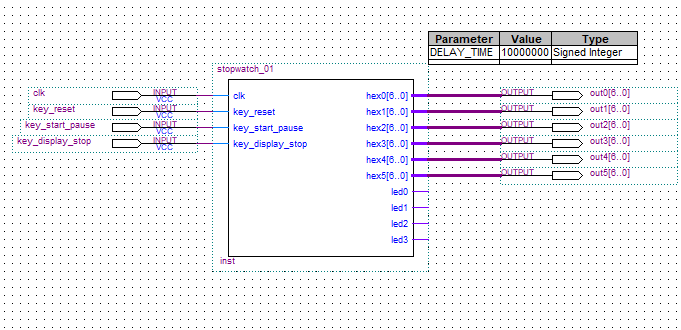
\includegraphics[width=\textwidth]{bdf.png}
            
        \subsection{verilog代码设计}
        	\par 详细请见代码注释。
            \par 计时主要是6个寄存器,分别代表毫秒高低位、秒高低位、分高低位,用多个if嵌套判断是否进位,最后一位的进位是直接清零。显示则是另外6个对应的寄存器,如果处于实时显示状态,则每次更新之前表示时间的寄存器后,把6个值赋给这6个用于显示的寄存器。
            \par 消抖的实现方式是记录之前的电位高低,随时与当前的电位高低对比,如果之前基本不是高电平,那么现在的低电平将不会导致状态的改变;现在的低电平只有在之前连续几个周期内是高电平时才会改变计时与显示的状态。当然reset复位不受影响,因为从肉眼效果来看几次高频率的复位可以基本等效成1次复位。
        
    \section{具体步骤}
    
    	\subsection{初始化} 设备驱动安装、在新建设备时选择实验设备的型号、设置时钟脉冲频率等。
        
        \subsection{实现代码} 根据设计要求把代码的主要功能部分全部实现,在给出的代码中自己填写的主要包括
        \par 1) 具体的6位数字更改解决方案
        \par 2) 计时状态更改、显示状态更改、复位解决方案
        \par 3) 消抖解决方案
        \par 具体代码实现请看本实验报告的第4部分\emph{完整代码}
        
        \subsection{完成BDF设计} 由于该实验只需要50MHz时钟频率,因此没有使用BDF中的pll模块,只使用了自己的verilog代码所生成的symbol,其中4个输入分别是时钟信号、复位、计时按钮、显示按钮,10个输出中6个是显像管,另外4个用于显示各种状态。
        
        \subsection{针脚分配} 对于输入的button和时钟信号每个都要分配1个针脚;对于输出的数字显像管每个都有7个针脚,按照实验手册进行匹配;由于实验未强制要求要使用LED灯,因此我没有对四个LED灯的输出进行针脚分配,如果需要的话,我觉得可以设置为电源状态、是否被复位、是否处于计时状态、是否实时显示计时。
        \subsection{编译与写入} 编译文件,通过编译后把内容烧写到FPGA板中。
    
    \section{完整代码}
    
    \par 注:由于latex排版代码不是很美观所以采用sublime编辑器并截图,如果需要完整代码,请至Github下载。我的Github地址https://github.com/yyong119/EI332SourceCode
    \par //**words**之中的注释是我认为比较关键的地方
	\newline
    \includegraphics[width=\textwidth]{1-40.jpg}
    \newline
    \includegraphics[width=\textwidth]{41-80.jpg}
    \newline
    \includegraphics[width=\textwidth]{81-120.jpg}
    \newline
    \includegraphics[width=\textwidth]{121-160.jpg}
    \newline
    \includegraphics[width=\textwidth]{161-end.jpg}


\end{document}
